% Preamble 
\documentclass[12pt]{report}
%\linespread{1.3}
\usepackage[utf8]{inputenc}
\usepackage[british,magyar]{babel} % korrekt elválasztás
\usepackage[T1]{fontenc} % korrekt elválasztás
\usepackage{t1enc} % ez, vagy a megelőző felesleges, de ha itt van mindkettő, az nem baj

\usepackage[a4paper, top=2.5cm,right=2.5cm,left=3cm,bottom=2.5cm]{geometry} 

\usepackage{appendix}

% Basics
\usepackage{color}
\usepackage{graphicx}
\usepackage{subcaption, caption}
\usepackage{float}
\usepackage{hhline}
\usepackage{wrapfig}
\usepackage{lipsum}
\usepackage{multirow}
\usepackage{{booktabs}}

	
% Links, quotes, fancies
\usepackage{tocbibind}

\usepackage[table]{xcolor}

\usepackage{url} 		% to include any web link.
\usepackage{listings}
\newcommand*{\rom}[1]{\expandafter\@slowromancap\romannumeral #1@}
\usepackage[final]{pdfpages}
\usepackage{datetime}  % to have month-year date type for the as of date.
\newdateformat{monthyeardate}{%
	\THEYEAR~\monthname[\THEMONTH]}

% Page style setup
\usepackage[raggedright, pagestyles]{titlesec}
\usepackage[raggedright]{titlesec}
\usepackage{fancyhdr}
\fancypagestyle{front}{%
	\fancyhf{}
	\renewcommand{\headrulewidth}{0pt}
	\fancyfoot[C]{\thepage}
}
\fancypagestyle{main}{%
	\fancyhf{}
	\fancyhead[R]{\rightmark}
	\fancyhead[L]{\leftmark}
	\fancyfoot[C]{\thepage}
	\renewcommand{\headrulewidth}{0.4pt} 
}
\fancypagestyle{plain}{%
	\fancyhf{}
	\fancyhead{}
	\fancyfoot[C]{\thepage}
	\renewcommand{\headrulewidth}{0pt}
}


\frenchspacing % magyar nyelvnek megfelelő mondatvégi térköz (pont utáni térköz csökkentése)
\linespread{1.3} 
\usepackage{indentfirst}

\usepackage{qrcode}

\usepackage{epigraph,varwidth}
\renewcommand{\epigraphsize}{\small}
\setlength{\epigraphwidth}{0.65\textwidth}
\renewcommand{\textflush}{flushepinormal}

%\usepackage{natbib}
\usepackage{import}
\usepackage[hidelinks]{hyperref}
\hypersetup{
	colorlinks,
	linkcolor={red!50!black},
	citecolor={blue!50!black},
	urlcolor={blue!80!black}
}  % reset the default color of hyperlinks

\makeatletter
\renewcommand{\sectionmark}[1]{\markright{\thesection~~~#1}}
\renewcommand{\chaptermark}[1]{\markboth{\if@mainmatter \fi#1}{}}
\makeatother

% % % renew abstract environment to avoid page renumberin
\makeatletter
\renewenvironment{abstract}{%
	\if@twocolumn
	\section*{\abstractname}%
	\else
	\small
	\begin{center}%
		{\bfseries \abstractname\vspace{-.5em}\vspace{\z@}}%
	\end{center}%
	\quotation
	\fi}
{\if@twocolumn\else\endquotation\fi}
\makeatother
\providecommand{\keywords}[1]{\small\textbf{Keywords: } #1}


% Doc Values

\title{\foreignlanguage{british}{Helpdesk} rendszer megvalósítása mikroszerviz alapú elosztott alkalmazással}
\author{Bőle Balázs}
\date{\today}
\graphicspath{{Figs/}}  % automatic graphics folder

%%%%%%%% DOCUMENT %%%%%%%%
\begin{document}
\sloppy
\pagenumbering{roman}
%%%% Title Page
%\pagestyle{empty}
\makeatletter  % referring to the values of title, etc.
\begin{titlepage}
\newcommand{\HRule}{\rule{\linewidth}{0.5mm}} 							% horizontal line and its thickness
\center 
%\flushright
% University
\textsc{\huge Gábor Dénes Főiskola}\\[1cm]

% Document info
\textsc{\LARGE Mérnökinformatikus alapképzés}\\[0.2cm]
\HRule \\[0.8cm]
{\huge \bfseries \@title}\\[0.7cm]								% Assignment
\HRule \\[2cm]

% Author
{\LARGE \bfseries
\@author}\\[1.5cm]
%Supervisor
{\Large Konzulens:\\[0.5cm]
Dr. Nagy Elemér Károly}\vspace{2cm}

{\LARGE Szoftverfejlesztés szakirány}\\[0.5cm]					    % Course Code


\includegraphics[height=0.2\textwidth]{gdf_logo.png}

\vfill
{\Large \monthyeardate{\@date}}
\end{titlepage}

\thispagestyle{empty}
\cleardoublepage

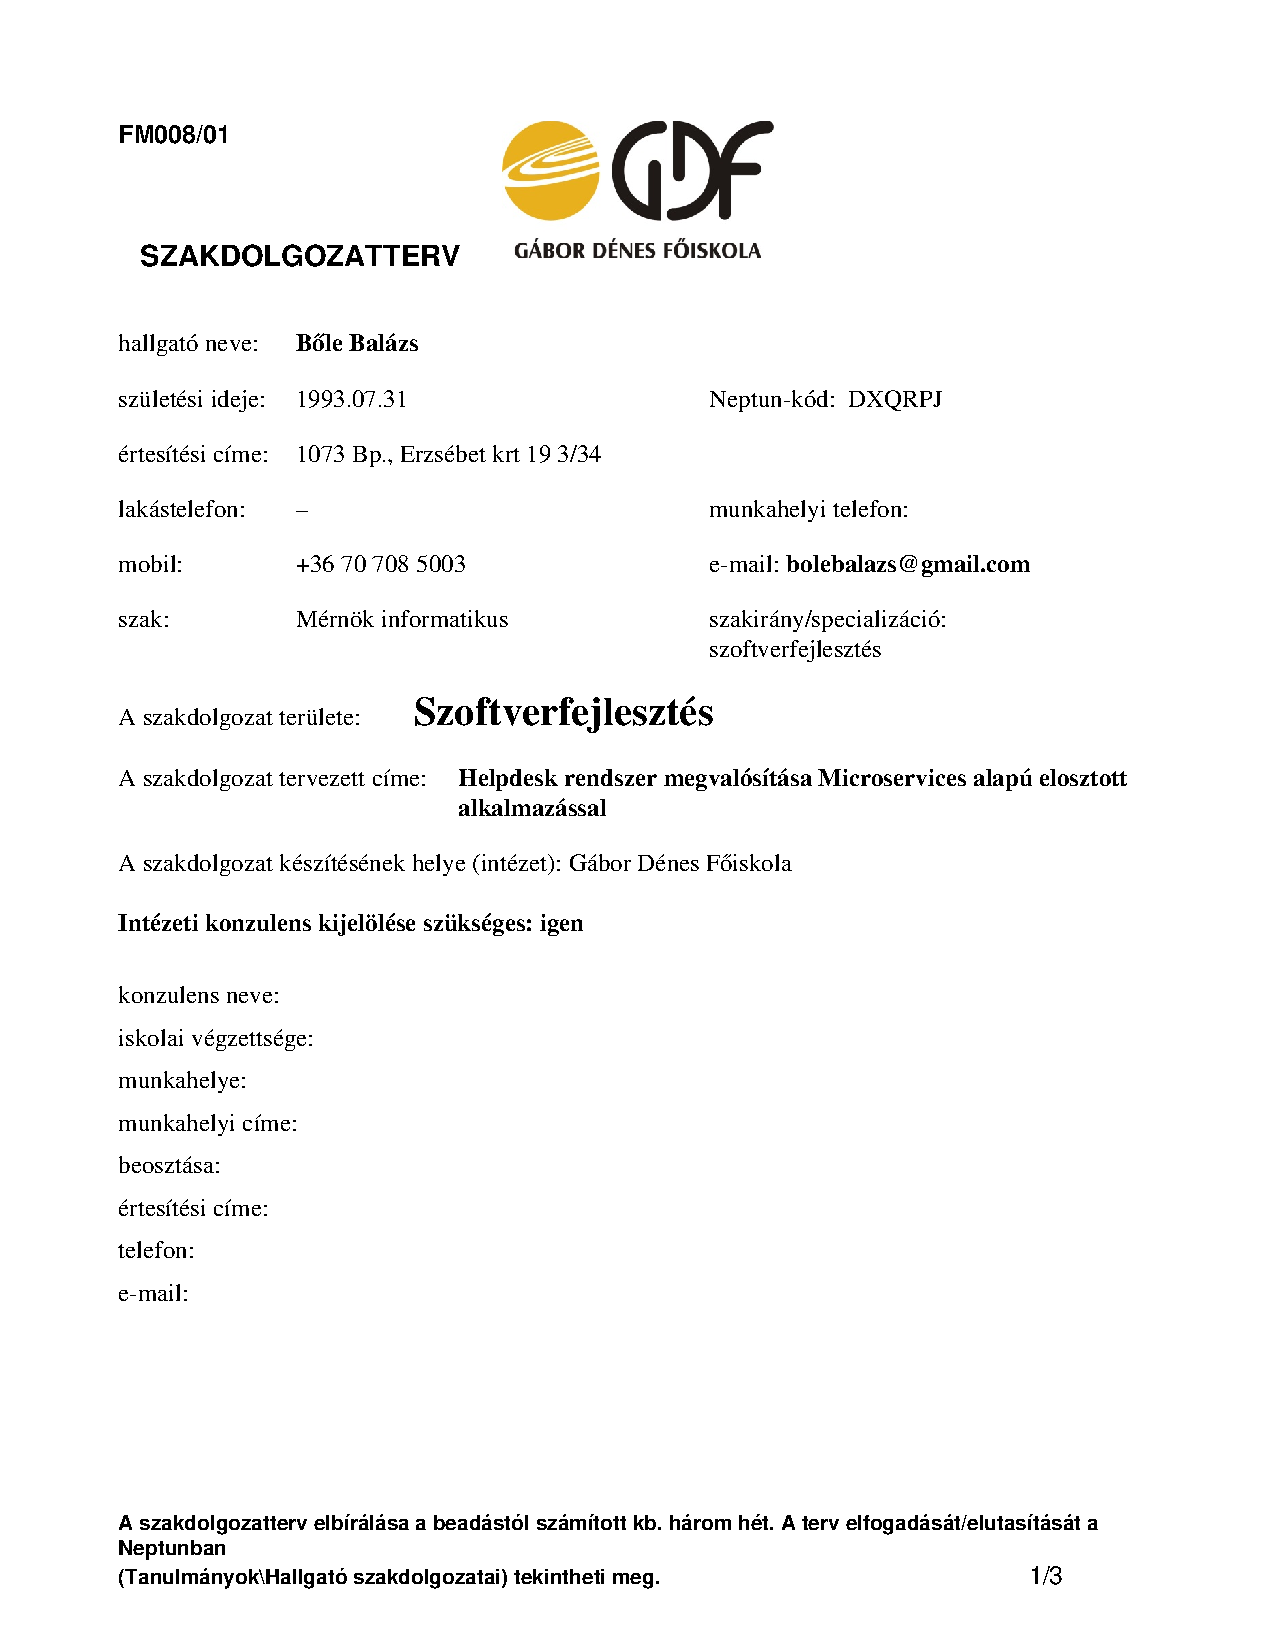
\includepdf[pages=-]{FM008_01_Szakdolgozatterv-DXQRPJ.pdf}
\cleardoublepage
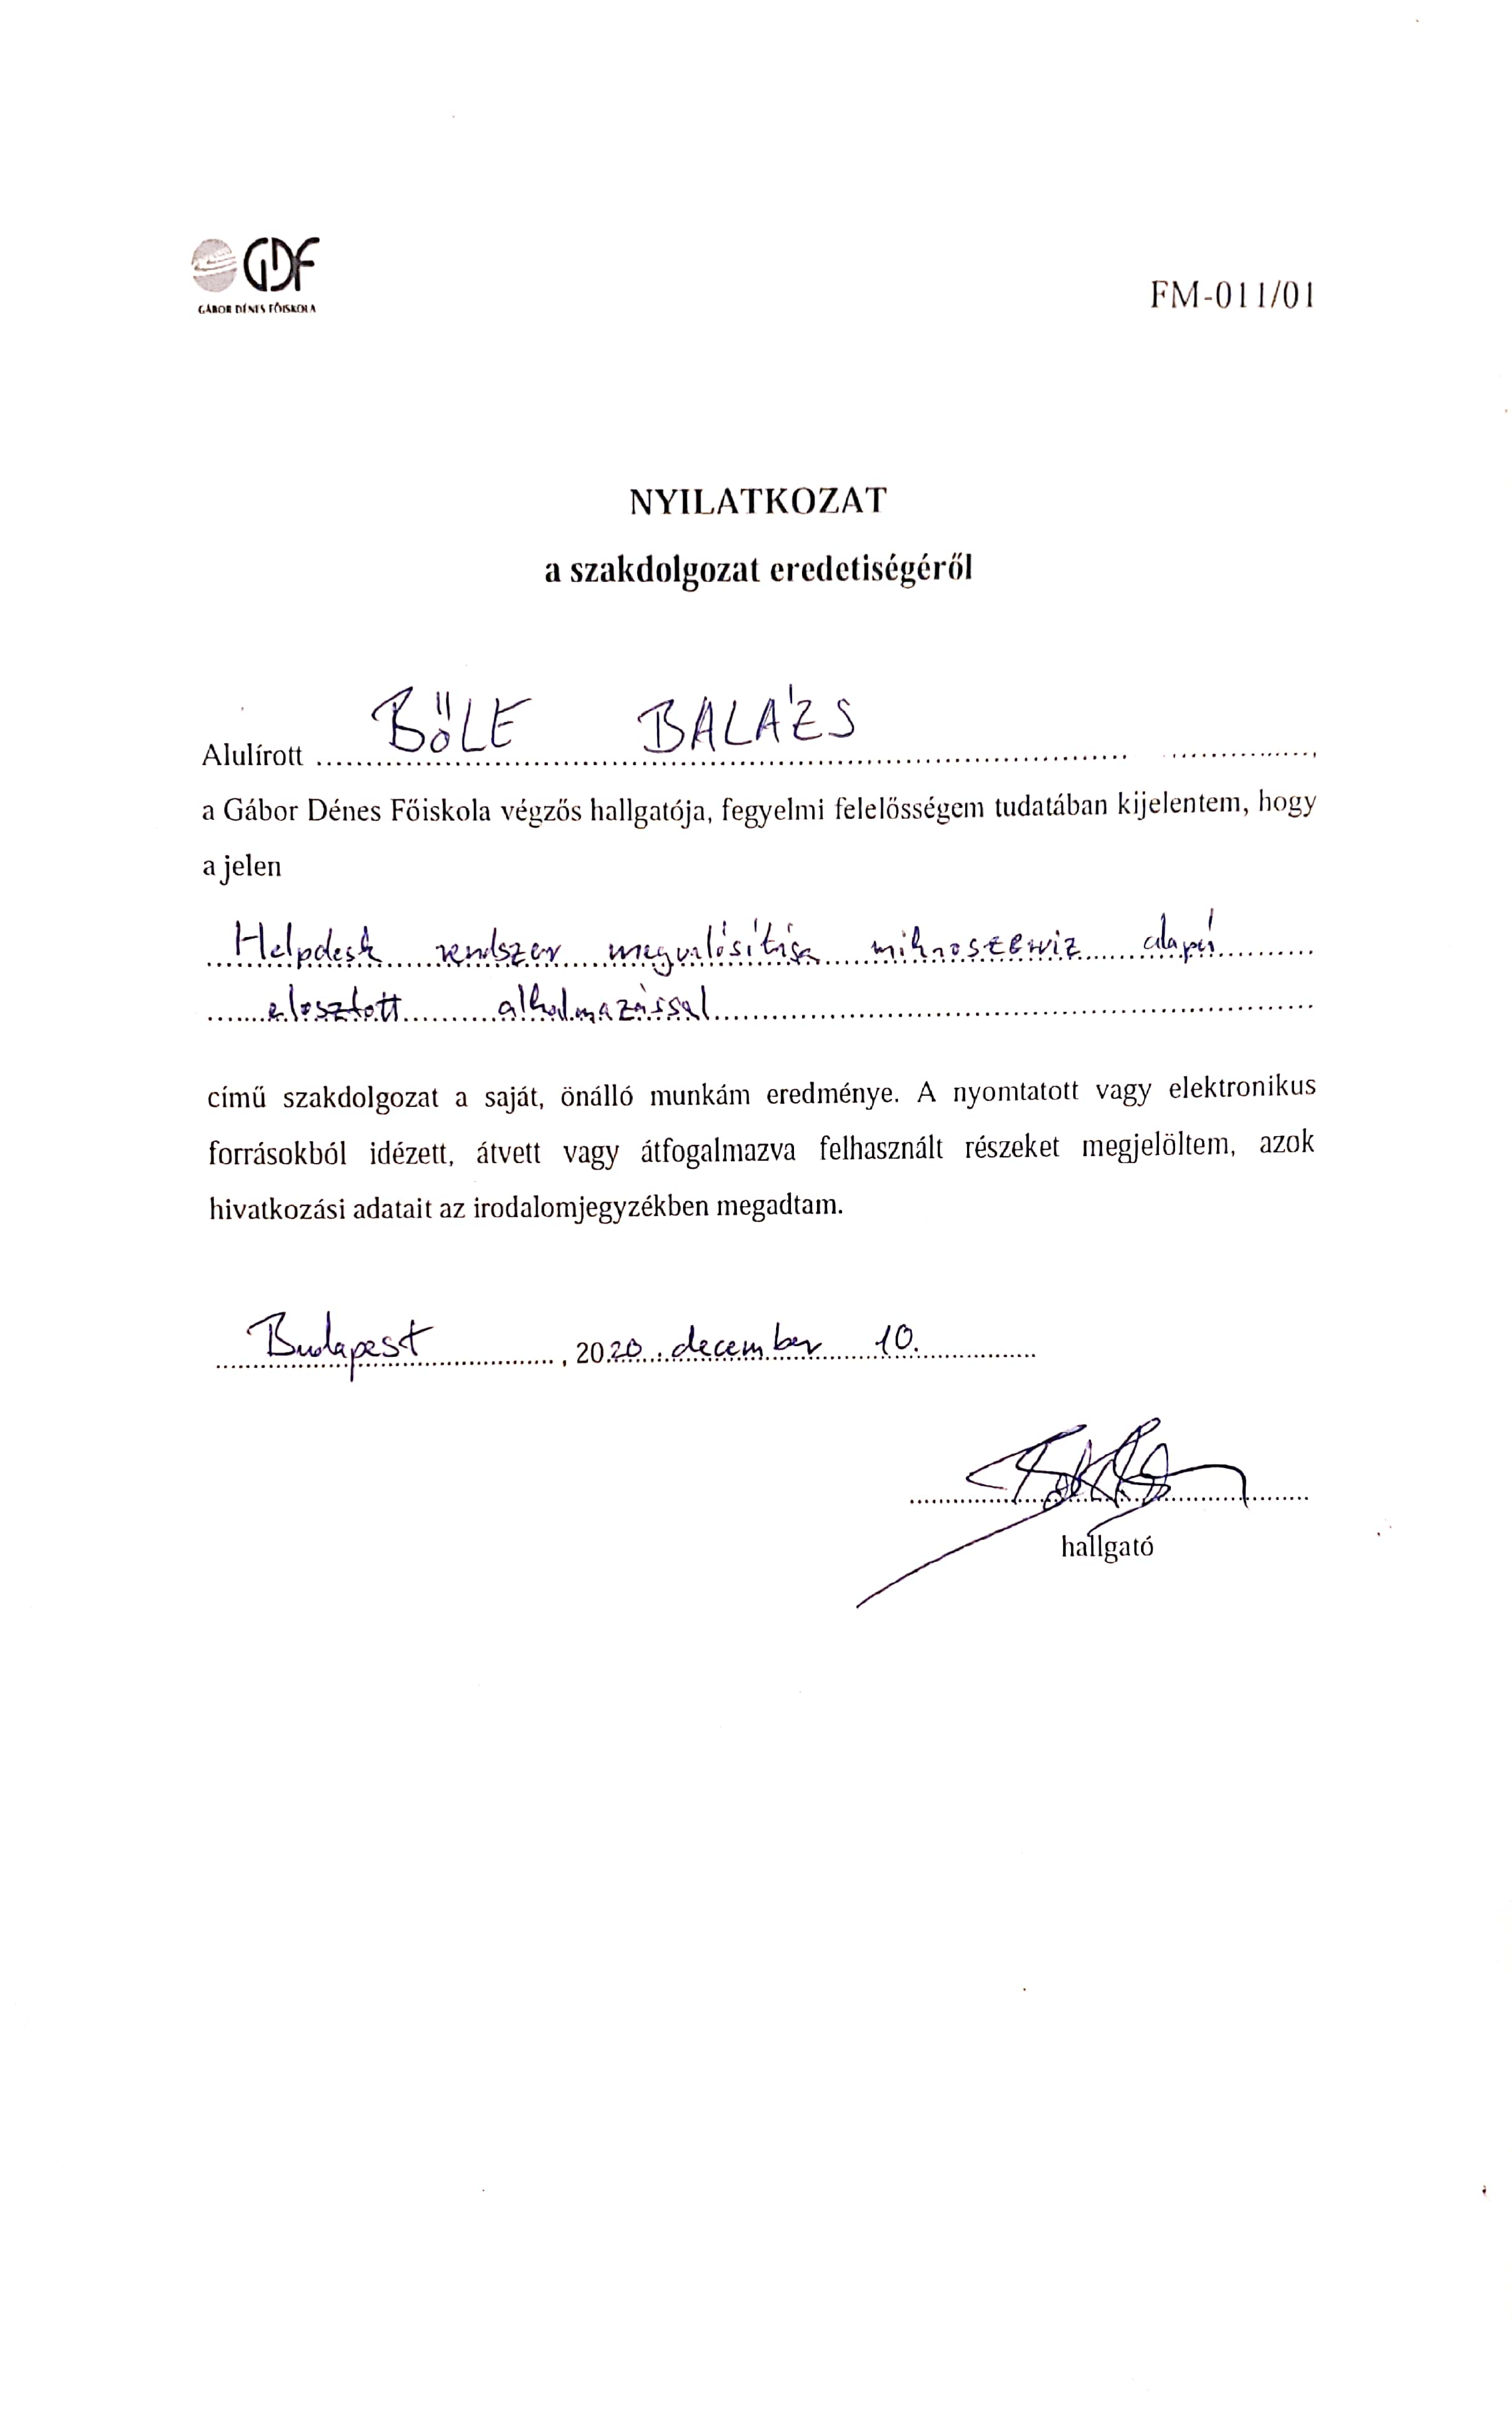
\includepdf[pages=-]{eredetiseg-nyilatkozat.pdf}

\thispagestyle{empty}
\cleardoublepage

\thispagestyle{empty}
\begin{center}
	{\Large \bfseries \@title}
	
	\bigskip
	\bigskip
	
	készítette
	
	\bigskip
	\bigskip
	
	{\large \bfseries \@author}
	
	\bigskip
	
	\vfill
	
	\begin{tabular}{ll}
		Neptun kód: & DXQRPJ \\
		Elérhetőség: & \href{mailto:bolebalazs@gmail.com}{bolebalazs@gmail.com}\\
		
		\bigskip\\
		
		Konzulens: & Dr.\ Nagy\ Elemér\ Károly
		

	\end{tabular}

	\bigskip
	\bigskip

\mbox{A dolgozat elektronikus változata elérhető a \url{https://github.com/balazsBole/} címen.}	
	

	
	\bigskip
	
	
\includegraphics[width=0.2\textwidth]{gdf_logo.png}

	
\end{center}
Budapest, \monthyeardate{\@date}.

\makeatother

\clearpage
\begin{abstract}
	Dolgozatomban ismertetem egy mikroszerviz alapú elosztott alkalmazás felépítését, a tervezés során fellépő általános problémákat, valamint ezekre a problémákra adható megoldásokat. 
	
	Nagy vonalakban és feladatspecifikusan áttekintem a felhasznált technológiákat és módszertanokat.
	
	Ezek tükrében bemutatom a létrehozott szoftvert,  infrastruktúrát és az üzemeltetéséhez szükséges eszközöket.
	
\end{abstract}

\pagestyle{front}
\tableofcontents

\begingroup
\let\clearpage\relax
\listoffigures
\endgroup


\clearpage
\pagenumbering{arabic}
\chapter*{Bevezetés}\label{ch:bevezetes}
	\addcontentsline{toc}{chapter}{\nameref{ch:bevezetes}}
Ahogy az \foreignlanguage{british}{O'Really} által az év elején készített felmérésből \cite{OReally} is látszik, a mikroszerviz alapú alkalmazások egyre nagyobb népszerűségnek örvendenek. Egyre több cég szeretné lecserélni meglévő monolit rendszerét, vagy a szükséges új funkciókat a régebbi rendszertől függetlenül, hibrid rendszerben valósítana meg.

Mint az a \foreignlanguage{british}{wiredelta} cikkéből \cite{wiredelta} is látszik, a mikroszerviz architektúrának számtalan előnye van. Míg a nagyvállalati környezetben sokszor a folyamatos szállítási igény, vagy az egymástól függetlenül fejleszthető alrendszerek miatt döntenek emellett a technológia mellett, az én esetemben a legfontosabb szerepet a skálázhatóság, az újrafelhasználhatóság, és  az alacsony fenntartási költség játszotta.

Úgy gondolom, hogy nincs olyan technológia, ami minden problémára megoldást nyújtana. De úgy érzem hogy az ilyen elvek mentén kialakított alkalmazások, természetükből adódóan időtállóbbak lesznek. Ha el tudjuk érni, hogy egy alkalmazás valóban csak egy funkcióért kell hogy felelős legyen, azzal a problémamegoldás analitikus oldalát  emeljük rendszerszintre. 

Éppen ezért, a mikroszerviz architektúra legnagyobb előnye szerintem a rendszerezésből következik.


\chapter{Üzleti igények}\label{ch:uzleti_igenyek}
\pagestyle{main}
\section{Funkcionális igények}



\section{Nem funkcionális igények}	



\chapter*{Diszkusszió}\label{ch:diszkusszió}
\pagestyle{plain}
Diszkusszió a végén
\lipsum


\newpage


% References
	\bibliographystyle{unsrturl}
\bibliography{references.bib}




\end{document}
